\section{Consensus layer support} \label{sec.consensus}

\subsection{The interlink pointers data structure}
\label{sec.interlink}

In order to construct our protocol, we rely on the same \emph{interlink data
structure} used by PoPoW~\cite{KLS}. This is an additional hash-based data
structure that is proposed to include in the header of each block. The
interlink data structure is a skip-list~\cite{skiplist} that makes it efficient
for a verifier to process a sparse subset of the blockchain, rather than only
consecutive blocks.

Valid blocks satisfy the proof-of-work condition: $id \leq T$, where $T$ is the
mining target. Throughout this work, we make the simplifying assumption that $T$
is constant. Some blocks will achieve a lower id. If $id \leq \frac{T}{2^\mu}$
we say that the block is of level $\mu$. All blocks are level $0$. Blocks with
level $\mu$ are called $\mu$-\textit{superblocks}. $\mu$-superblocks for $\mu >
0$ are also $(\mu - 1)$-superblocks. The level of a block is given as $\mu =
\left \lfloor \log(T) - \log(\sf{id}(B)) \right \rfloor$ and denoted
$\textit{level}(B)$. By convention, for $Gen$ we set $id = 0$ and $\mu =
\infty$.

Observe that in a blockchain protocol execution it is expected half of the
blocks will be of level $1$, $1/4$ of the blocks will be of level $2$, $1/8$
will be of level $3$ and $1/2^\mu$ blocks will be of level $\mu$. In
expectation, the number of superblock levels of a chain $\chain$ will be
$\Theta(\log(\chain))$~\cite{KLS}. Figure~\ref{fig.hierarchy} illustrates the
blockchain superblocks starting from level $0$ and going up to level $3$ in case
these blocks are distributed exactly according to expectation. Here, each level
contains half the blocks of the level below.

In our protocol, the verifier must roughly scan along one level at a time. To
enable this, instead of just the previous block, the interlink vector also
points to the most recent preceding block of every level $\mu$. Genesis is of
infinite level and hence a pointer to it is included in every block at the first
available index within the interlink data structure. The number of pointers that
need to be included per block is in expectation $\log(|\chain|)$.

Figure~\ref{fig.hierarchy} illustrates the blockchain superblocks starting from
level $1$ and going up to level $4$ in case these blocks are distributed
exactly according to expectation. Note that each level contains half the blocks
of the level below.

\begin{figure}
    \caption{The hierarchical blockchain.
    Higher levels have achieved a lower target (higher difficulty) during mining.}
    \centering
    \iftwocolumn
        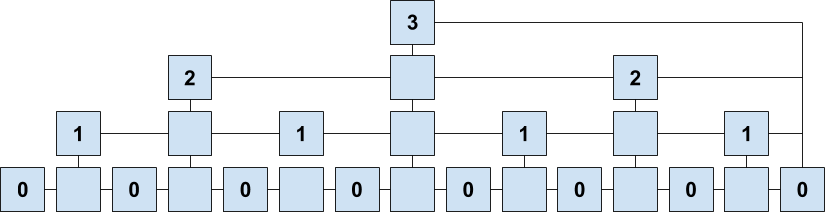
\includegraphics[width=0.9\columnwidth,keepaspectratio]{figures/hierarchical-ledger.png}
    \else
        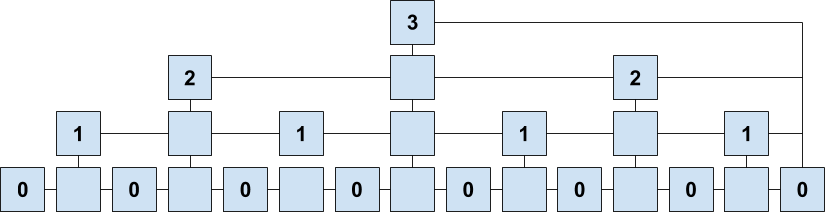
\includegraphics[width=0.7\columnwidth,keepaspectratio]{figures/hierarchical-ledger.png}
    \fi
    \label{fig.hierarchy}
\end{figure}

The algorithm for this construction is shown in
Algorithm~\ref{alg.nipopow-interlink} and is borrowed from~\cite{KLS}. The
interlink data structure turns the blockchain into a
skiplist-like~\cite{skiplist} data structure.

The updateInterlink algorithm accepts a block $B'$, which already has an
interlink data structure defined on it. The function evaluates the
interlink data structure which needs to be included as part of the next block.
It copies the existing interlink data structure and
then modifies its entries from level $0$ to $\textsf{level}(B')$ to
point to the block $B'$.

\import{./}{algorithms/alg.nipopow-interlink.tex}

\noindent\textbf{Traversing the blockchain. }
As we have now extended blocks to contain multiple pointers to previous blocks,
if certain blocks are omitted from a chain we will obtain a subchain, as long as
the blockchain property that each block must contain a pointer to its previous
block in the sequence is maintained.

Blockchains are sequences, but it is more convenient to use set notation for
some operations. Specifically, $B \in \chain$; $\chain_1 \subseteq \chain_2$ and
$\emptyset$ have the obvious meaning. $\chain_1 \cup \chain_2$ is the chain
obtained by sorting the blocks contained in both $\chain_1$ and $\chain_2$ into
a sequence (this may be not always defined).
We will freely use set builder notation $\{B \in \chain: p(B)\}$.
$\chain_1 \cap \chain_2$ is the
chain $\{B: B \in \chain_1 \land B \in \chain_2\}$. In all cases, the
blockchain property must be maintained. The lowest common ancestor is
$\textsf{LCA}(\chain_1,
\chain_2) = (\chain_1 \cap \chain_2)[-1]$.
If $\chain_1[0] = \chain_2[0]$ and $\chain_1[-1] = \chain_2[-1]$, we say the
chains $\chain_1, \chain_2$ \textit{span} the same block range.

It will soon become clear that it is useful to construct a chain containing only
the superblocks of another chain. Given $\chain$ and level $\mu$, the
\textit{upchain} $\chain\upchain^\mu$ is defined as $\{B \in \chain: level(B)
\geq \mu\}$. A chain containing only $\mu$-superblocks is called a
$\mu$\textit{-superchain}. It is also useful, given a $\mu$-superchain $\chain'$
to go back to the regular chain $\chain$. Given chains $\chain' \subseteq
\chain$, the \textit{downchain} $\chain'\downchain\!\!_\chain$ is defined as
$\chain[\chain'[0]:\chain'[-1]]$. $\chain$ is the \textit{underlying chain} of
$\chain'$. The underlying chain is often implied by context, so we will simply
write $\chain'\downchain$. By the above definition, the $\chain\upchain$
operator is absolute: $(\chain\upchain^\mu)^{\mu + i} = \chain\upchain^{\mu +
i}$. Given a set of consecutive rounds $S = \{r, r + 1, \cdots, r + j\}
\subseteq \mathbb{N}$, we define $\chain^S = \{B \in \chain: B \text{ was
generated during } S\}$.
